\documentclass{beamer}
%\usetheme{Ilmenau}
%\usecolortheme{beaver}

\usepackage[slovak,american]{babel}
\usepackage[utf8]{inputenc}
\usepackage{graphicx}
\usepackage{adjustbox}
 \usepackage{xcolor}
 
 \newsavebox\MBox
\newcommand\Cline[2][red]{{\sbox\MBox{$#2$}%
  \rlap{\usebox\MBox}\color{#1}\rule[-2.2\dp\MBox]{\wd\MBox}{1pt}}}

%\usefonttheme{serif}

%\definecolor{UKOrange}{HTML}{ef9424} %
\definecolor{UKOrange}{HTML}{7a2c18} %
\definecolor{UKBrown}{HTML}{a96d5e} %
\definecolor{UKLight}{HTML}{d8b6ab} %
\definecolor{UKDark}{HTML}{7a4f44}
\definecolor{UKDarker}{HTML}{4d312b} 
\definecolor{UKDarkest}{HTML}{2e1e1a}
\definecolor{UKRed}{HTML}{bf1f1c}

\setbeamertemplate{footline}[frame number]{}
\setbeamertemplate{navigation symbols}{}

%\usecolortheme{beaver}
\setbeamertemplate{itemize item}[square]
\setbeamercolor{itemize item}{fg = UKBrown}
\setbeamercolor{itemize subitem}{fg = UKLight}
\setbeamercolor{enumerate item}{fg = UKDark}

\setbeamercolor{footnote}{fg=UKLight}
\setbeamercolor{footnote mark}{fg=UKLight}
\setbeamerfont{footnote}{size=\tiny}
\renewcommand\footnoterule{}

\usetheme{default}
\beamertemplatenavigationsymbolsempty
\setbeamercolor{title}{fg=white, bg=UKBrown}
\setbeamercolor{frametitle}{fg=white, bg=UKBrown}
\setbeamercolor{block title}{bg=UKBrown, fg= white}
\setbeamercolor{block body}{bg =UKLight, fg = UKDarkest}

\setbeamercolor{block title alerted}{bg=UKOrange, fg= white}
\setbeamercolor{block body alerted}{bg =UKLight, fg = UKDarkest}


%\setbeamercolor{section in toc}{fg = UKBrown}
%\setbeamercolor{section in toc}{fg = UKDarkest}

% odstrani gulicky
\renewcommand*{\slideentry}[6]{}

\useoutertheme[subsection=false]{miniframes}
\AtBeginSection[]{\subsection{}}

\setbeamercolor{below lower separation line head}{bg=UKDark}
\addtobeamertemplate{headline}{}{%
  \begin{beamercolorbox}[colsep=0.5pt]{below lower separation line head}
  \end{beamercolorbox}
}
%\setbeamercolor*{mini frame}{fg=white,bg=UKRosy}
\setbeamercolor{section in head/foot}{fg=UKLight, bg=UKDark}

\usepackage{etoolbox}
\makeatletter
\preto{\@verbatim}{\topsep=0pt \partopsep=0pt }
\makeatother

%\setbeamertemplate{itemize/enumerate body begin}{\normalsize}
%\setbeamertemplate{itemize/enumerate subbody begin}{\normalsize}




%\newcommand{\codeblock}[2]{ \begin{block}{#1} \begin{verbatim}#2\end{verbatim}\end{block}}

%\defbeamertemplate*{title page}{customized}[1][]
%{
%  \begin{centering}
%    \begin{beamercolorbox}[sep=8pt,center]{title}
%      \usebeamerfont{title}\inserttitle
%    \end{beamercolorbox}
%  \end{centering}
%  \bigskip
%
%\begin{columns}[onlytextwidth,T]
%
%
%  \column{27mm}
%  \includegraphics[width=27mm]{images/logoFMFI.png}
%  
%  \column{\dimexpr\linewidth-54mm-6mm}
%  \centering
%  \vspace{5mm}  
%  \usebeamerfont{author}\insertauthor\par
%  \vspace{5mm}
%  \usebeamerfont{institute}\insertinstitute\par
%
%  \column{27mm}
%  \includegraphics[width=27mm]{images/logoUK.png}  
%\end{columns}
%\centering
%\vspace{7mm}
%  \usebeamerfont{date}\insertdate\par
%}

\DeclareMathOperator*{\argmin}{arg\,min}
\newcommand{\e}[1]{$\cdot 10^{#1}$}

%\newcommand{\codeblock}[2]{ \begin{block}{#1} \begin{verbatim}#2\end{verbatim}\end{block}}



\title[3. cvičenie]{Pokročilé spracovanie obrazu - Farebné priestory}
\author[Kocur]{Ing. Viktor Kocur \\{\small viktor.kocur@fmph.uniba.sk}}
\institute{DAI FMFI UK}
\date{9.10.2019}

\begin{document}
\selectlanguage{slovak}

\begin{frame}
  \titlepage
\end{frame}

%\begin{frame}
%  \tableofcontents
%\end{frame}

\section{Farby}
\subsection{HSV}
\begin{frame}
\frametitle{HSV}
  \begin{block}{HSV}
  HSV je farebný model orientovaný na intuitívne využite (tzv. uživateľský model). Hue predstavuje pozíciu na farebnom kruhu (odtieň), saturation je sýtosť a value je jas. 
  \end{block} 
  
  \begin{block}{rgb2hsv}
  rgb2hsv(I) - vráti obraz zapísaný v podľa HSV modelu, má rovnaké rozmery ako I, tj. tiež má tri kanály.
  \end{block} 
  
    \begin{block}{hsv2rgb}
  hsv2rgb(I\_hsv) - urobí to isté ale naopak.
  \end{block} 
\end{frame}

\begin{frame}
\frametitle{HSV - Úloha}
  \begin{block}{HSV}
  Použite GUI z minula. Ale namiesto R, G a B sliderov to budú H, S, V slidre. Telo funkcie bude skoro rovnaké obrázok, ale musíte najprv premeniť na HSV, upraviť a potom konvertovať na RGB.
  \end{block} 

  \begin{block}{GUI}
  Ak nemáte uložené GUI, tak si môžete stiahnuť súbory z minulého cvika a upraviť gui\_sliders.m.
  \end{block}   
\end{frame}

\subsection{CIE Lab}
\begin{frame}
\frametitle{CIE Lab}
  \begin{block}{CIE Lab}
  CIE L* a* b* je model s troma zložkami. L predstavuje jas (luminance), a je pozícia na ose zelená-červená a b je pozícia na ose modrá-žltá.
  \end{block} 

  
  \begin{block}{rgb2lab}
  rgb2lab(I) - vráti obraz zapísaný v podľa CIE Lab modelu, má rovnaké rozmery ako I, tj. tiež má tri kanály.
  \end{block} 
  
    
  \begin{block}{lab2rgb}
  lab2rgb(I\_lab) - urobí to isté ale naopak.
  \end{block} 

  
  \begin{block}{Úloha}
  Upravte gui, tak aby slidre reprezentovali zložky L, a, b.
  \end{block} 
\end{frame}

\subsection{CMY a CMYK}

\begin{frame}
\frametitle{RGB}
  \begin{block}{RGB}
  RGB je aditívny model, tj. na čierne pozadie pridávame farby. Ak prídáme všetky tri farby, tak vznikne biela farba. 
  \end{block} 

  \begin{center}
  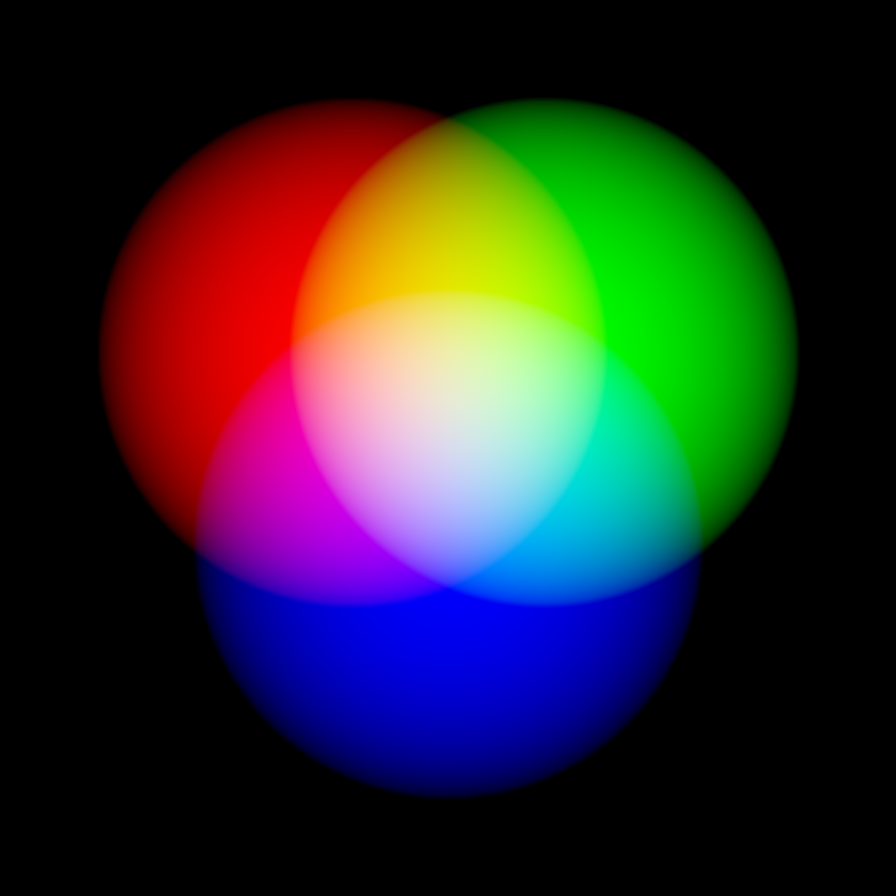
\includegraphics[height=0.5\textheight]{RGB.png}
  \end{center}
\end{frame}

\begin{frame}
\frametitle{CMY}
  \begin{block}{CMY}
  CMY je substraktívny model, tj. na biele pozadie pridávame farby. Ak prídáme všetky tri farby, tak vznikne čierna farba. 
  \end{block} 

  \begin{block}{CMYK}
  CMYK má navyše čiernu farbu. To je vhodné pre tlačiarne. 
  \end{block} 

  \begin{center}
  
\includegraphics[height=0.5\textheight]{CMY.png}
  \end{center}
\end{frame}

\begin{frame}
\frametitle{CMY vs. RGB}
  \begin{block}{CMY}
  Pre farbý podľa CMY a RGB platí prechod C~=~255~-~R, M~=~255~-~G a Y~=~255~-~B
  \end{block} 
  
  \pause

  \begin{block}{RGB}
  Naopak platí R = M + Y, G = C + Y, B = C + M
  \end{block} 
\end{frame}

\begin{frame}
\frametitle{Euklidovská vzdialenosť}
  \begin{block}{Úloha}
  Napíšte skript ktorý zobrazí obrázok farby,png. Pomocou funkcie ginput vyberte tri body a zistite aká je vzdialenosť medzi prvým a zvyšními dvoma pre rôzne farebné modely. Porovnajte, či podobné farby sú pri sebe bližšie ako zdanlivo rôzne farby.
  \end{block} 
  
    \begin{block}{Euklidovská vzdialenosť}
  \begin{equation*}
  \rho_e(\vec{a}, \vec{b}) = \sqrt{\sum_{i=1}^n (a_i - b_i)^2}
  \end{equation*}
  \end{block} 

  \begin{block}{ginput}
  [x ,y] = ginput(n) - vráti vektory x-ových a y-ových súradníc bodov na ktoré užívateľ po zadaní príkazu klikne vo figure
  \end{block} 
\end{frame}


\section{Indexované obrázky a pseudofarby}
\subsection{Pseudofarby}
\begin{frame}[fragile]
\frametitle{Pseudofarby}
  \begin{block}{Pseudofarby}
  Pseudofarby využijeme na zafarbenie šedotónového obrázka, tak aby sa zvýraznili niektoré detaily.
  \end{block} 
  
  \begin{block}{colormap}
  colormap(mapa) - zmení farby ktorými sa vykresluje obrázok na tie ktoré sú v mape. Mapa môže byť buď prednastavená (jet, hsv, winter, copper, bones, gray...), alebo matica $n \times 3$, kde na každom riadku je RGB trojica, ktorá predstavuje farbu.
  \end{block} 

  \begin{block}{Kód}
  \begin{verbatim}
  BW = imread('medical.pgm');
  imagesc(BW);
  colormap(hsv);\end{verbatim}
  \end{block} 
\end{frame}

\subsection{Indexované obrázky}
\begin{frame}[fragile]
\frametitle{Indexované obrázky}
  \begin{block}{Indexovaný obrázok}
  Indexovaný obrázok je taký, v ktorom každý pixel nieje reprezentovaný vlastnou RGB farbou, ale indexom. Tento index ukazuje ktorá farba sa v danom pixely nachádza. Na to však aby bolo jasné ktorý index korešponduje k akej farbe je nutné mať mapu farieb, tj. maticu $n \times 3$, kde na každom riadku je RGB trojica a $n$ je počet indexovaných farieb.
  \end{block} 
\end{frame}

\begin{frame}[fragile]

  \begin{block}{rgb2ind}
  [X, map] = rgb2ind(I,n) - vráti indexovaný obraz X (podobný label matici) s n farbami a mapu $n \times 3$ tj. zoznam trojíc farieb v poradí podľa ktorého sa indexuje. \\
    X = rgb2ind(I,map) - vráti indexovaný obraz X pre danú mapu.
  \end{block}   
  
  
    \begin{block}{imhist}
  hist = imhist(X,map) - vráti histogram, tj. vektor početností pre jednotlivé indexy. V prípade, že si výstup nikam neuložíme, tak sa histogram nakreslí.
  \end{block} 
  
  \begin{block}{Kód}
  \begin{verbatim}
   [X, map] = rgb2ind(I,30);
   imagesc(X);
   colormap(map);
   figure;
   imhist(X,map);\end{verbatim}
  \end{block} 
\end{frame}


\begin{frame}
\frametitle{Úloha}    
  \begin{block}{Úloha}
  Obrázok zátišia prekonvertujte na indexovaný pre 20 farieb a zistite, ktorá z týchto farieb je dominantná (nájdite jej RGB trojicu). K tomu aj zistite koľko percent pixelov má práve túto farbu.
  \end{block}   
  
  \begin{block}{Hint}
  Pomôže vám príkaz max, pozrite si ho v helpe.
  \end{block}  
  
  \begin{alertblock}{Pozor!}
  Pre prípad ak nepoužijete funkciu imhist, tak je dôležité si uvedomiť, že indexy v obrázku začínaju na 0, ale indexy v mape začínajú 1!
  \end{alertblock}   
\end{frame}



\end{document}